% Подписи колонтитула
\newcommand{\colontitulAutors}{astronom\_v\_cube}
\newcommand{\colontitulYear}{2022}
\newcommand{\colontitulEducationalSubject}{Теория колебаний}
\newcommand{\colontitulTeacher}{Некоркин В.И.}

%Настройки шаблона
\documentclass[10pt,landscape,a4paper]{article}
\usepackage[utf8]{inputenc}
\usepackage[english, russian]{babel}
\usepackage[T1,T2A]{fontenc}  
\usepackage{upgreek} % прямые греческие ради русской традиции
\usepackage{tikz}
\usetikzlibrary{shapes,positioning,arrows,fit,calc,graphs,graphs.standard}
%\usepackage[nosf]{kpfonts}
%\usepackage[t1]{sourcesanspro}
\usepackage{multicol}
\usepackage{wrapfig}
\usepackage[top=6mm,bottom=8mm,left=4mm,right=4mm]{geometry}
\usepackage[framemethod=tikz]{mdframed}
\usepackage{microtype}
\usepackage{pdfpages}
\usepackage{amsthm,amsmath,amscd}   % Математические дополнения от AMS
\usepackage{amsfonts,amssymb}       % Математические дополнения от AMS
\usepackage{mathtools}              % Добавляет окружение multlined
\usepackage{xfrac}                  % Красивые дроби
\usepackage{physics}

\usepackage{fancyhdr} % колонтитулы

%некоторые математические команды
\newcommand{\Div}{\operatorname{div}}
\newcommand{\Grad}{\operatorname{grad}}

\let\bar\overline

\definecolor{myblue}{cmyk}{1,.72,0,.38}

\def\firstcircle{(0,0) circle (1.5cm)}
\def\secondcircle{(0:2cm) circle (1.5cm)}

\colorlet{circle edge}{myblue}
\colorlet{circle area}{myblue!5}

\tikzset{filled/.style={fill=circle area, draw=circle edge, thick},
	outline/.style={draw=circle edge, thick}}

\pgfdeclarelayer{background}
\pgfsetlayers{background,main}

%\everymath\expandafter{\the\everymath \color{myblue}}
\everydisplay\expandafter{\the\everydisplay \color{myblue}}

\renewcommand{\baselinestretch}{.8}
\pagestyle{empty}

\global\mdfdefinestyle{header}{%
	linecolor=gray,linewidth=1pt,%
	leftmargin=0mm,rightmargin=0mm,skipbelow=0mm,skipabove=0mm,
}

\makeatletter % Author: ttps://tex.stackexchange.com/questions/218587/how-to-set-one-header-for-each-page-using-multicols
\renewcommand{\section}{\@startsection{section}{1}{0mm}%
	{.2ex}%
	{.2ex}%x
	{\color{myblue}\sffamily\small\bfseries}}
\renewcommand{\subsection}{\@startsection{subsection}{1}{0mm}%
	{.2ex}%
	{.2ex}%x
	{\sffamily\bfseries}}

\makeatother
\setlength{\parindent}{0pt}

%колонтитулы
\pagestyle{fancy}
\fancyhf{}
\setlength{\headheight}{40pt}
\setlength{\headsep}{4pt}
\renewcommand{\headrulewidth}{1pt}
\fancyhead[L]{\textcopyright~\colontitulAutors}
\fancyhead[C]{Программа минимум по курсу <<\colontitulEducationalSubject>> \colontitulYear г}
\fancyhead[R]{Преподаватель:~\colontitulTeacher}

\begin{document}
	\small
	\begin{multicols*}{2}
		\section{Определение динамической системы}
		
		\section{Условия грубости динамических систем на плоскости}
		Так как динамические системы изменяются вместе со входящими в них параметрами, но при малости изменений качественные черты поведения сохраняются, вводится свойства грубости. Грубость — устойчивость структуры разбиения фазовой плоскости динамических систем на траектории по отношению к малым изменениям динамической системы.\\
		Для плоскости: пусть есть система:\\
		$\begin{cases}
			\dot{x} = P(x,y) \\
			\dot{y} = Q(x,y)
		\end{cases} $\\
		где $P$ и $Q$ - гладкие функции, система диссипативна.\\
		Система — грубая, если существует число $\delta>0$, что все динамические системы вида:\\
		$\begin{cases}
			\dot{x} = P(x,y) + p(x,y) \\
			\dot{y} = Q(x,y) + q(x,y)
		\end{cases} $\\
		в которых аналитические функции удовлетворяют условию $\left\lvert p(x,y)\right\rvert  + \left\lvert q(x,y)\right\rvert  $, имеют такую же структуру разбиения на положительные полутраектории, что и начальная система.\\
		Переход от одной грубой ДС к другой происходит через негрубую ДС.\\
		ДС на прямой устойчива (структурно грубая), если для всех состоянии равновесия $\lambda_i(\mu)\neq 0$.

		\section{Бифуркация состояний равновесия динамических систем на прямой}
		Значение параметра, при котором ДС является негрубой, называется бифуркационным.

		\section{Метод линеаризации определения устойчивости состояний равновесия}

		\section{Линейный осциллятор. Основные свойства}

		\section{Резонанс в линейном осцилляторе}

		\section{Определение предельного цикла. Характеристики}

		\section{Автоколебания и автоколебательная система. Мягкий и жесткий режимы возбуждения}
		Автоколебательная система — диссипативная система, совершающая незатухающие колебания при отсутствии колебательного воздействия извне. В этих системах возникает баланс между действиями диссипативных потерь и внутренних механизмов, компенсирующих потери. Автоколебания — незатухающие колебания в нелинейной диссипативной системе, форма и свойства которых в определенных пределах не зависит от начальных условий и определяется параметрами самой системы.\\
		1. Мягкий режим\\
		2. Жесткий режим\\
		\textbf{Свойства автоколебательных систем}\\
		$\divideontimes$ Источник энергии для компенсации диссипации — постоянен и находится внутри самой системы\\
		$\divideontimes$ Система содержит колебательную подсистему и активный нелинейный элемент\\
		$\divideontimes$ В изолированной колебательной системе происходят затухающие колебательные процессы, а активный элемент может усиливать колебания и их нелинейно ограничивать\\
		$\divideontimes$ Между колебательной подсистемой активным элементом существует обратная связь, регулирующая поступление энергии от источника\\
		$\divideontimes$ Автоколебания в определенных пределах не зависят от начальных условиях и определяются параметрами системы\\
		$\divideontimes$ Математическим образом периодических автоколебаний является предельной цикл

		\section{Бифуркационные сценарии рождения периодических движений динамических систем на плоскости}
		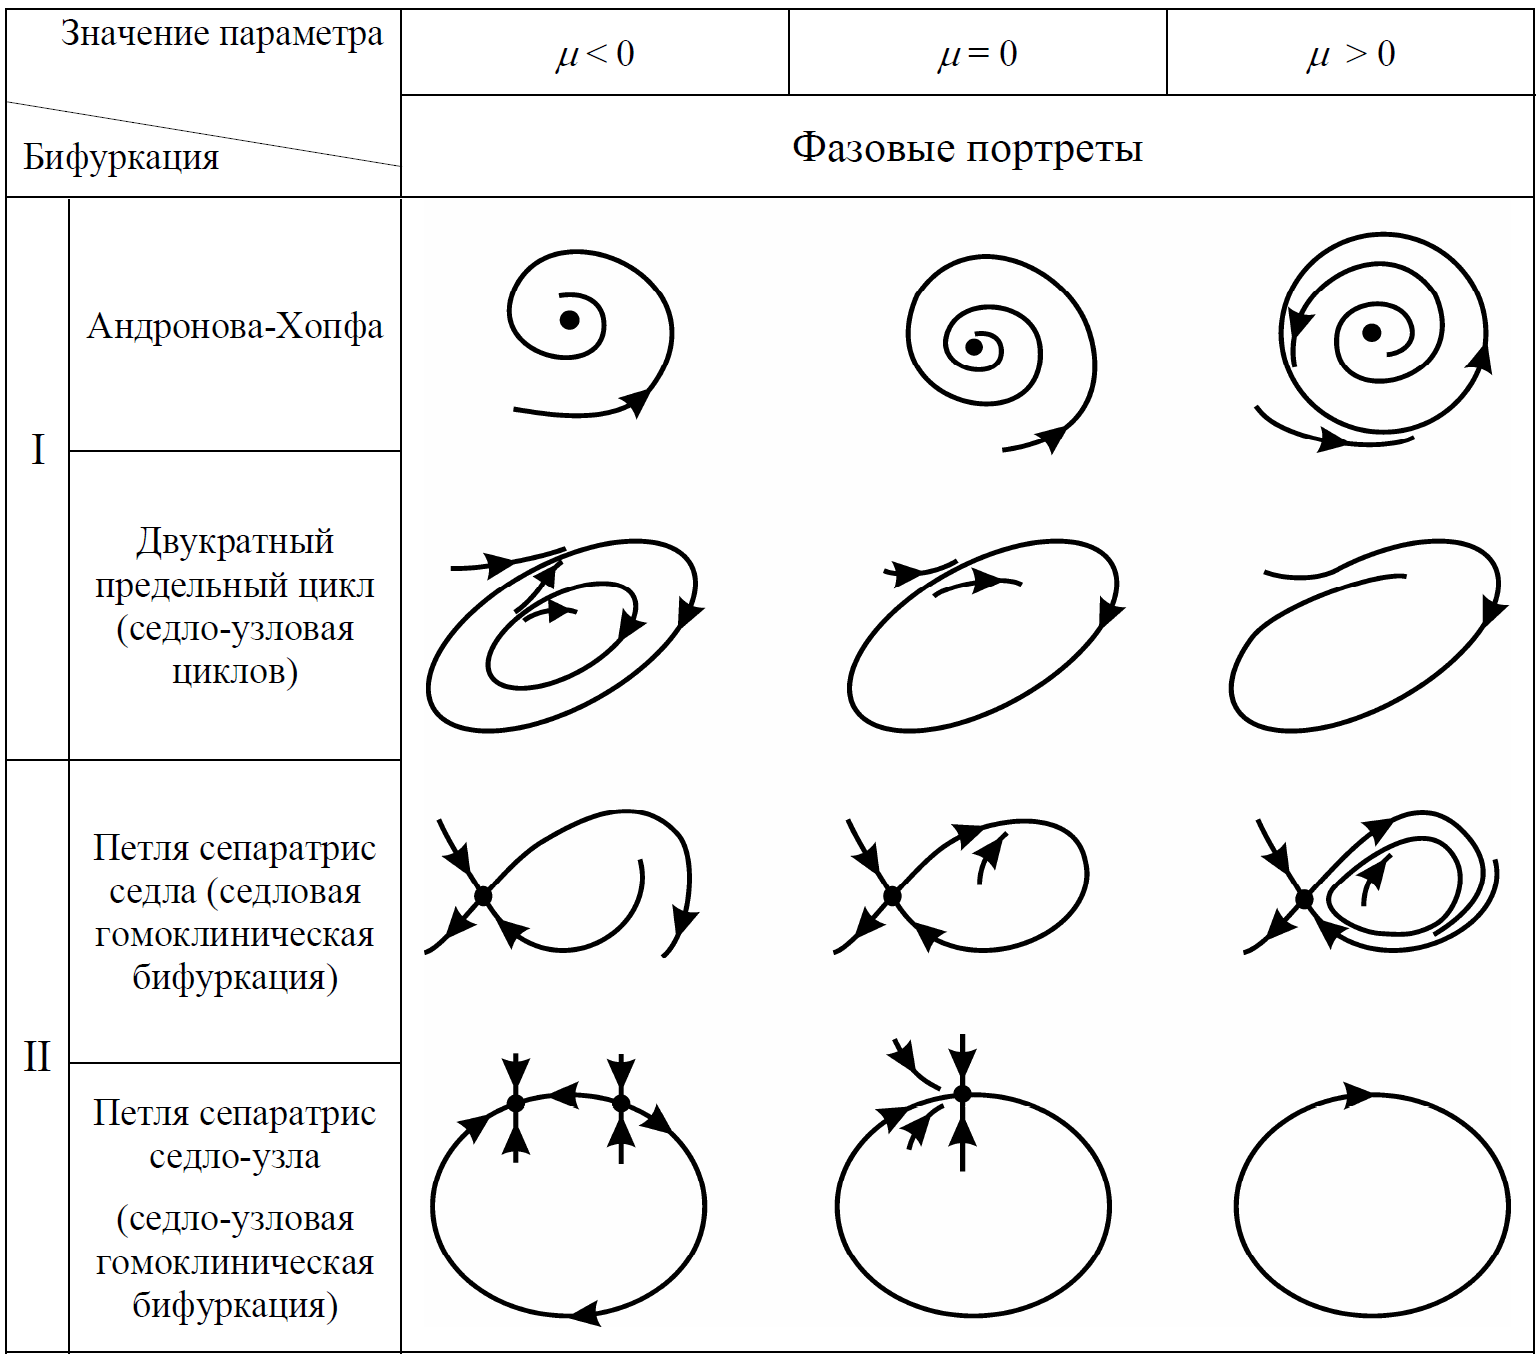
\includegraphics[width=0.75\linewidth]{tk_img/bifurk.png}

		\section{Дисперсия, ее физическая природа и проявления}
		Дисперсия — зависимость фазовой скорости волны от ее частоты. Связь между частотой и волновым числом гармонической волны определяется пространственными и временными масштабами среды и называется дисперсионным соотношением.\\

		\begin{tabular}{|l|c|}
			$\omega^2 = {\omega_0}^2 + \dfrac{4\gamma }{m}sin^2(\dfrac{ka}{A})$\\
			$a$ - расстояние между маятниками\\ $\gamma$ - жесткость пружины\\ $k$ - действительное волновое число\\ & 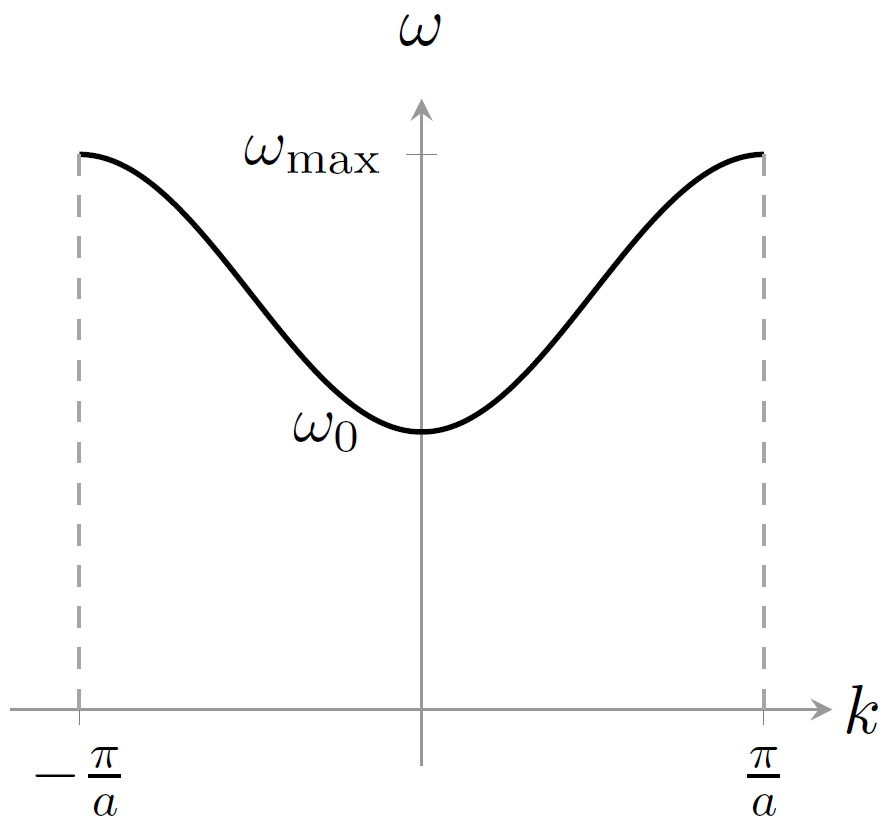
\includegraphics[width=0.45\linewidth]{tk_img/dispers.png}\\
		\end{tabular}
		
		У каждой компоненты волнового пакета будет своя $V_\text{ф}$, возникает его деформация. Наличием собственных масштабов объясняется эффект частичного непропускания волны\\
		Область прозрачности: $k\in Re$ - распространение без искажения гармонической волны\\
		Область непрозрачности: $k\in Im$ - нераспространение.

		\section{Простые волны. Основные свойства и условия существования}
		$U_t + C(U)U_x = 0$ — нелинейное уравнение простой волны. $C(U)$ — дифференцируемая функция (скорость от состояния среды). Характеристики — линии, вдоль которых переменная $U(x, t)$ будет оставаться постоянной и равной по значению для каждого соответствующего значения $x$.\\
		В точке пересечения характеристик их значения одинаковы — появится точка разрыва (производная равна $infty$) -  градиентная катастрофа. На переднем фронте образуется ударная волна. Уравнение перестает работать после точки разрыва.

		\section{Параметрические системы. Основные свойства}
		Параметрически системы — системы, где внешнее воздействие находится внутри системы и может изменять ее параметры.\\
		\textbf{Резонансные. } Период изменения параметров находится в целочисленном соотношении с периодом собственных колебаний. В такт с изменением энергии, соответствующей собственным колебаниям, вносится энергия, вызванная работой внешнего воздействия. При определенных условиях может привести к эффекту раскачки колебаний за счет накапливающейся в системе энергии. \\
		\textbf{Нерезонансные. }Параметры изменяются очень быстро или очень медленно в сравнении с характерными временными масштабами изменения переменных системы.\\
		\textbf{Свойства.}\\
		1. Параметрическая система, находящаяся в начальный момент в состоянии равновесия, останется в этом состоянии при $t>0$ (дергая за нитку, маятник нельзя раскачать)\\
		2. Состояния равновесия параметрической системы могут быть как устойчивы, так и неустойчивы\\
		3. Если параметры системы таковы, что она неустойчива и система выведена из состояния равновесия, то в ней возникают колебания, амплитуда которых $\uparrow exp$.Процесс возрастания размаха в колебаний при периодическом нарастании колебаний — параметрический резонанс.

		\section{Релаксационные колебания}

		\section{Локальные бифуркации состояний равновесия трехмерных систем}

		\section{Локальные бифуркации периодических движений трехмерных систем}

	\end{multicols*}
\end{document}
